\documentclass[
  journal=pasa,
  manuscript=research-paper, %% or "review"
  year=2021,
  volume=37,
]{cup-journal}

\usepackage{microtype,siunitx,booktabs}

\DeclareRobustCommand{\VAN}[3]{#2}
\let\VANthebibliography\thebibliography
\def\thebibliography{\DeclareRobustCommand{\VAN}[3]{##3}\VANthebibliography}

%%%%% AUTHORS - PLACE YOUR OWN PACKAGES HERE %%%%%
\usepackage{graphicx}	% Including figure files
\usepackage{amsmath}	% Advanced maths commands
\usepackage{amssymb}	% Extra maths symbols
\usepackage{xspace}

%%%%%%%%%%%%%%%%%%%%%%%%%%%%%%%%%%%%%%%%%%%%%%%%%%

%%%%% AUTHORS - PLACE YOUR OWN COMMANDS HERE %%%%%
% STELLAR LABELS
\newcommand{\Teff}{$T_\mathrm{eff}$\xspace}
\newcommand{\logg}{$\log g$\xspace}
\newcommand{\feh}{$\mathrm{[Fe/H]}$\xspace}
\newcommand{\numax}{$\nu_\mathrm{max}$\xspace}
\newcommand{\vmic}{$v_\mathrm{mic}$\xspace}
\newcommand{\vsini}{$v \sin i$\xspace}
\newcommand{\vrad}{$v_\mathrm{rad}$\xspace}

% NAMES
\newcommand{\TheCannon}{\textit{The Cannon}\xspace}
\newcommand{\sme}{\textsc{sme}\xspace}
\newcommand{\marcs}{\textsc{marcs}\xspace}
\newcommand{\Gaia}{\textit{Gaia}\xspace}
\newcommand{\TLF}{\Teff, \logg, and \feh}

% UNITS
\newcommand{\dex}{\,\mathrm{dex}}	% dex
\newcommand{\K}{\,\mathrm{K}}	% dex
\newcommand{\Msol}{\,\mathrm{M_\odot}} % Msol
\newcommand{\kpc}{\,\mathrm{kpc}}	% kpc
\newcommand{\yr}{\,\mathrm{yr}}	% Gyr
\newcommand{\Gyr}{\,\mathrm{Gyr}}	% Gyr
\newcommand{\eV}{\,\mathrm{eV}}	% eV
\newcommand{\Angstroem}{\,\text{\AA}}	% Angstroem
\newcommand{\kms}{\,\mathrm{km\,s^{-1}}}	% km/s
\newcommand{\kpckms}{\,\mathrm{kpc\,km\,s^{-1}}}	% kpc km/s
\newcommand{\kmkmss}{\,\mathrm{km^2\,s^{-2}}}	% km^2/s^2
\newcommand{\kmsMpc}{\,\mathrm{km\,s^{-1}\,Mpc^{-1}}}	% km/s/Mpc

\sisetup{detect-all,separate-uncertainty=true}

\title{The GALAH Survey: Data Release 4}

\author{S. Buder}
\affiliation{Research School of Astronomy \& Astrophysics, Australian National University, Canberra, ACT 2611, Australia}
\affiliation{ARC Centre of Excellence for All Sky Astrophysics in 3 Dimensions (ASTRO 3D), Australia}
\email[S. Buder]{sven.buder@anu.edu.au}

\author{The GALAH Collaboration}
% \alsoaffiliation{Joint first authors}

%\handlingeditor{Excellent E Editor}

\doi{10.1017/pasa.2020.32}

\received {dd Mmm YYYY}
\revised  {dd Mmm YYYY}
\accepted {dd Mmm YYYY}
\published{22 September 2020}

\keywords{
Surveys; the Galaxy; methods: observational; methods: data analysis; stars: fundamental parameters; stars: abundances} %% First letter not capped
% \jel{Q11; Q12; D81; M31}
% \msc{Q14; Q18; E21}
% \abbreviations{
%     BDHS: Bangladesh Demographic and Health Survey, 
%     IDA: Fe-deficiency anaemia, 
%     IFA: Fe-folic acid, 
%     MNP: multiple micronutrient powder, 
%     VAD: vitamin A deficiency
% }

\begin{document}

\begin{abstract}
In this data release, we aim to estimate even more accurate and precise elemental abundances of the 30 elements with absorption features in GALAH spectra by using as much information of the spectra as possible. This includes the previously neglected molecular absorption features of $\mathrm{C_2}$ and CN, who can only be analysed with a self-consistent grid of synthetic spectra.

In this release, we us Bayesian Markov-Chain Monte-Carlo (MCMC) framework that is fitting all 30+ parameters at the same time and uses prior information on stars in the form of non-spectroscopic data from \Gaia (e.g. parallaxes), 2MASS (e.g. infrared magnitudes), and K2 (e.g. \numax).

To achieve a self-consistent grid of synthetic spectra, we compute significantly over-sampled synthetic spectra at 10- times higher then the typical GALAH resolution with Spectroscopy Made Easy (\sme). The stellar parameters (\Teff, \logg, \feh, \vmic) and elemental abundances [X/Fe] of all 30 elements are randomly sampled within reasonable limits (e.g. $\pm 1 \dex$ for most [X/Fe]) and fed into \sme to create self-consistent synthetic spectra over the full wavelength range for \marcs atmospheres.

To limit computational costs of the randomly drawn MCMC samples, we employ a novel method: We select 2076 reasonably small 3-dimensional bins in the \sme grid, that is \Teff$= \pm 500\K$, \logg$ = \pm 0.5\dex$, and \feh$ = \pm 0.5\dex$ and train a quadratic \TheCannon model for each of these bins. We select the bins so that they overlap in all 3-dimensions and allow us to find a reasonably smooth interpolation between different bins / \TheCannon models. In this step, we also apply different rotational broadening and add them as a label for \TheCannon. For each combination of \Teff, \logg, and \feh of the MCMC sampler, we quickly lookup the nearest-neigbhor model of \TheCannon with a KD-tree method and create a synthetic spectrum with \TheCannon. These high-resolution synthetic spectra are then degraded with the measured resolution profile of each spectrum.

The MCMC fitting algorithm further fits for \vrad the following nuisance labels: starting wavelength of each CCD (not degenarate with \vrad if more than 1 CCD are fitted), dispersion of each CCD.

Normalised spectra of the spectroscopic analysis (not to be confused with the output of the reduction pipeline) are produced by Chebychev fits to the ratio of observed and synthetic spectra and can thus take into account significant changes to the flux due to molecular absorption features (thus becoming independent of the notoriously difficult search for continuum points).

Abundance measurements are confirmed by assessing the significance of flux changes through changes of the specific element abundance in \TheCannon model compared to the signal-to-noise.

We run the pipeline in 5 different setups:
- use only spectroscopic information (in case asteroseismic or parallax informations are unreliable)
- use non-spectroscopic information
- assume the spectrum to be part of a binary system and fit a flux ratio q, 2 rv, 2 teff, 2 logg, 2 feh (currently only an idea)
\end{abstract}

\section{INTRODUCTION}

\section{REDUCTION}

Outcome of reduction pipeline:
\begin{table}
    \centering
    \caption{Data product 1: FITS files of reduced spectra}
    \label{tab:reduction_fits}
    \begin{tabular}{c|c}
    \hline \hline
    FITS Ext. & Description \\
    \hline
    Ext. 0 & Un-normalised spectrum \\
    Ext. 1 & Normalised spectrum (by reduction pipeline) \\
    Ext. 2 & ? \\
    Ext. 3 & ? \\
    Ext. 4 & ? \\
    Ext. 5 & ? \\
    Ext. 6 & ? \\
    Ext. 7 & FWHM Resolution profile \\
    \hline
    \end{tabular}
\end{table}

\section{ANALYSIS}

Similar to \citet{Rix2016}

Optimised normalisation by chebychev fit to synthesis/observation: can take molecular features into account and overcome issue of balmer line normaliazion function in SME!

Add fit to wavelength solution - simply cdelt1 and crval1 but 1 global rv?

Can figure out if detection by simply adjusting specific [X/Fe] in Cannon model and see how spectrum reacts compared to SNR

\subsection{Workflow}

\subsection{Grid of synthetic spectra from \sme}

\begin{figure}[hbt!]
 \centering
 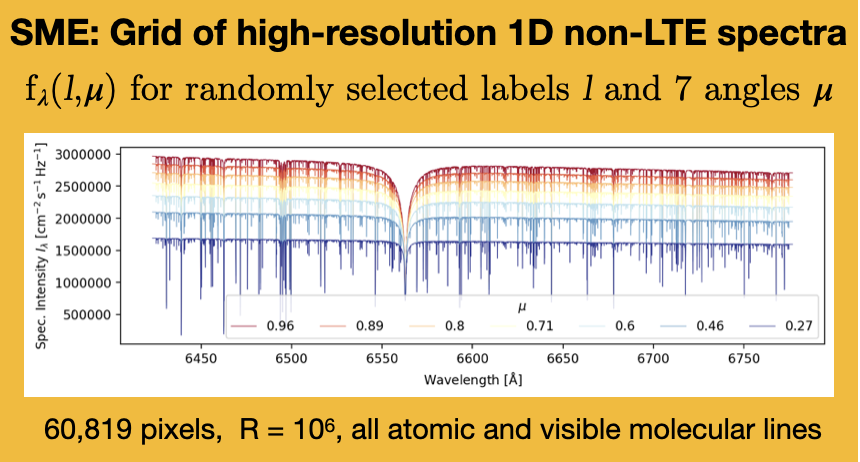
\includegraphics[width=\columnwidth]{figures/sme_grid.png}
 \caption{Explanation of SME grids}
 \label{fig:sme_grid}
\end{figure}

For each spectrum, we 

For each spectrum, we first run a test on all available lines in the GALAH linelist, which is adapted from \citet{Heiter2021} and includes small changes to correct wrong $\log gf$ values for few lines within the GALAH wavelength range. We keep all atomic lines for the final synthesis and restrict the molecular lines to those with \textsc{sme}.depth above 0.001.

Spectra are computed at a resolution of $R = 1,000,000$ on a fine wavelength grid with 60,819 pixels spread over the extended wavelengths $4675.1- 4949.9$, $5624.1-5900.9$, $6424.1-6775.9$, and $7549.1-7925.9 \Angstroem$. We note that these extend significantly beyond the actual GALAH wavelength range.

Default inputs are the grids of 1D \marcs atmospheres \citep[][version 2014]{Gustafsson2008}, which are interpolated for the choice of \Teff, \logg, and \feh. We use grids of non-LTE departure coefficients by \citet{Amarsi2020} for H, Li, C, N, O, Na, Mg, Al, Si, K, Ca, Mn, and Ba.

We compute the fluxes for 7 equal-area midpoints of equal-area annulii and save them for the later disk integration under consideration of different rotational broadening \vsini (see Sec.~\ref{sec:cannon_input}).

\subsection{Synthetic spectrum interpolation via \TheCannon}

\begin{figure}[hbt!]
 \centering
 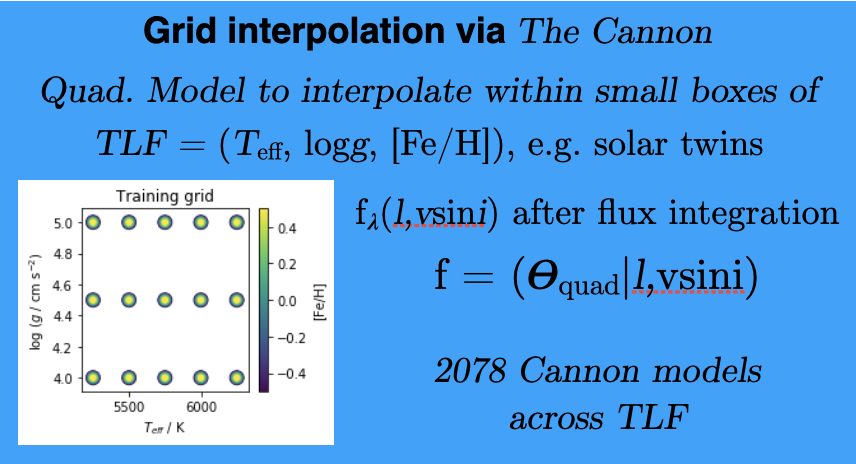
\includegraphics[width=\columnwidth]{figures/cannon_interpolation.png}
 \caption{Explanation of cannon interpolation}
 \label{fig:cannon_interpolation}
\end{figure}

We are training 2067 models for overlapping 3D bins in \Teff, \logg, and \feh.

\subsubsection{Training \TheCannon} \label{sec:cannon_input}

We have a sample of synthetic spectra $f_\lambda (\mu)$ that lay within each 3D bin of \TLF. These cover different choices of \TLF as well as \vmic and [X/Fe], but are assuming no rotational broadening. We therefore add an additional label, \vsini~$\in~[2.5, 5, 10, 15, 30] \kms$.

\subsubsection{Creating synthetic spectra for a set of labels} \label{sec:cannon_synthesis}

For each combination of \TLF, we finding \TheCannon's nearest neighbor model via \textsc{scipy} \textsc{cKDTree}.

\subsection{Fitting routine}

\subsection{Available and used information}

\begin{itemize}
    \item observed flux $f_\text{obs}$ for each wavelength
    \item uncertainty of observed flux $\sigma_\text{obs}$ (assumed to be Gaussian) for each wavelength
\end{itemize}

Available but not used:
\begin{itemize}
    \item $\varpi$ and its uncertainty from the astrometric solution
    \item Optical photometry $G_\text{BP}$, $G$, $G_\text{RP}$ and their uncertainties from \Gaia eDR3 \citep{Brown2021}
    \item Near-infrared photometry $J$, $H$, $K_s$ and their uncertainties from 2MASS \citep{Skrutskie2006}
    \item Infrared photometry $W_1$ - $W_4$ from WISE \citep{Cutri2013}
    \citep{Lindegren2021a} of \Gaia eDR3 \citep{Brown2021}, including a zeropoint correction by \citet{Lindegren2021b}
    \item \numax and its uncertainty from K2 \citep[][in prep.]{Zinn2020}
    \item $\delta \nu$ and its uncertainty from K2 \citep[][in prep.]{Zinn2020}
\end{itemize}

\subsubsection{Bayesian Framework}

\textbf{Posterior}
\begin{align}
    \ln p (l \vert f_\text{obs}, \sigma_\text{obs})
    \propto
    \ln p (l) + \ln p (f_\text{obs} \vert \sigma_\text{obs}, l)
\end{align}

\textbf{Likelihood}
\begin{align}
    \ln p \left( f_\text{syn} \vert f_\text{obs}, l \right) = - \frac{1}{2} \left[ \frac{\left(f_\text{syn}(l) - f_\text{obs} \right)^2}{\sigma_\text{obs}} \right]
\end{align}

\textbf{Priors}

Prior on \logg from \numax etc.?

\begin{align}
    p (l) = \begin{cases} 0 \\ 1 \end{cases}
\end{align}

\subsubsection{MCMC}

\subsubsection{Nuisance fitting along the way}


\begin{figure}[hbt!]
 \centering
 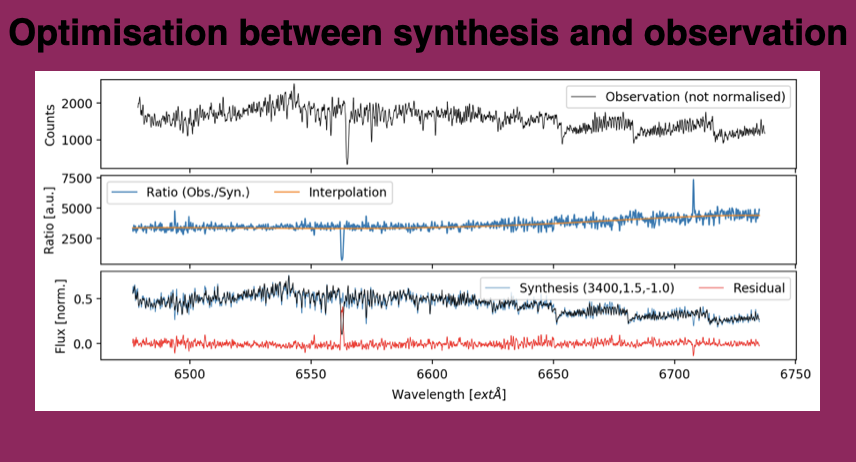
\includegraphics[width=\columnwidth]{figures/ratio_normalisation.png}
 \caption{Explanation of normalisation}
 \label{fig:ratio_normalisation}
\end{figure}

Chebychev polynomials are fitted between each synthetic spectrum from Sec.~\ref{sec:cannon_synthesis}

\section{VALIDATION}

Flag if parameters outside of the range of \TheCannon (e.g. \vsini$ > 30 \kms$, see Sec.~\ref{sec:cannon_input})

\section{Conclusions}

\section*{Acknowledgements}


% \begin{table*}
% \begin{threeparttable}
% \caption{Identified backscatter from objects in orbit and their properties}\label{satdet}
% \begin{tabular}{ c c c c c c } \toprule
% Satellite\tnote{a}   &NORAD           &Start      &End               &Mean intensity         &RCS\tnote{b}            \\
% name        &ID \#           &time (UT)       &time (UT)             & (Jy/beam)      &($m^{2}$)        \\ \midrule
% BGUSAT      & 41999 &2020-01-31 14:40:09.9  &2020-01-31 14:43:11.9  &1060  &$<$0.1       \\ 
% ISS (ZARYA) & 25544 &2020-01-31 17:17:41.9  &2020-01-31 17:19:00.9  &440  & $>$1.0      \\ 
% MAX VALIER SAT& 42778 &2020-02-03 01:18:16.9  &2020-02-03 01:20:09.9  &650  &0.1 $-$ 1.0       \\
% ISS (ZARYA) &22554 &2020-02-03 01:31:07.9  &2020-02-03 01:33:14.9  &930  &$>$1.0         \\ 
% FLOCK 3P 71 & 42024 &2020-02-01 14:16:22.9& 2020-02-01 14:18:05.9  &330  &$<$0.1       \\ 
% ISS (ZARYA) & 25544 &2020-02-02 02:18:17.9  &2020-02-02 02:20:16.9  &740  &$>$1.0 \\  
% BGUSAT      & 41999 &2020-02-02 02:18:17.9  &2020-02-02 02:20:16.9  &1010  &$<$0.1 \\ \bottomrule
% \end{tabular}
% \begin{tablenotes}
% \item[a] TLE information for predicted trajectories from space-track.org for the epoch of observation: 2020-02-01
% \item[b] Radar Cross Section (RCS) is categorised by space-track.org as: small ($<$0.1); medium (0.1 $<$ RCS $<$ 1.0); and large ($>$1.0)
% \end{tablenotes}
% \end{threeparttable}
% \end{table*}

% PASA uses footnotes, not endnotes. \endnote in this template will behave like \footnote; and \printendnotes will not output anything.
% \printendnotes

\bibliography{bib}

\appendix

% \section{Hospital Anxiety and Depression Scale (Italian Version)}

% \section{Openness to Discuss Cancer in the Family Scale Questionario sulla Comunicazione in Famiglia (Italian Version)}

% \begin{table}[hbt!]
% \centering
% \begin{threeparttable}
% \caption{Predicting approval of one's own house member}\label{tab:predictapproval}
% \begin{tabular}{lSSS}
%   \toprule
%   & {(1)} & {(2)} & {(3)} \\
%   \midrule
%   Religion Match & 0.077\tnote{***} & -0.029 & -0.027 \\
%                   & {(0.014)} & {(0.061)} & {(0.062)} \\
%   \bottomrule
% \end{tabular}
% \begin{tablenotes}[para]
%   \item[]Note: Entries are coefficients from a probit regression model. Robust standard errors in parentheses.
%   \item[***] $p < 0.01$,
%   \item[**] $p < 0.05$,
%   \item[*] $p < 0.1$, two-tailed test.
% \end{tablenotes}
% \end{threeparttable}
% \end{table}


\end{document}
